\documentclass[10pt,pdf]{beamer}
\usepackage[T2A]{fontenc}
\usepackage[utf8]{inputenc}%включаем свою кодировку: koi8-r или utf8 в UNIX, cp1251 в Windows
\usepackage[english,russian]{babel}%используем русский и английский языки с переносами
\usepackage{amssymb,amsfonts,amsmath,mathtext,cite,enumerate,float} %подключаем нужные пакеты расширений

\usepackage{color}

\newcommand*{\mathcolor}{}
\def\mathcolor#1#{\mathcoloraux{#1}}
\newcommand*{\mathcoloraux}[3]{%
  \protect\leavevmode
  \begingroup
    \color#1{#2}#3%
  \endgroup
}

\renewcommand{\theenumii}{.\arabic{enumii}}% Меняем везде перечисления на цифра.цифраx

\renewcommand{\theenumiii}{.\arabic{enumiii}}% Меняем везде перечисления на цифра.цифра
\title[Ядерные методы в детектировании аномалий\hspace{8mm} \insertframenumber/\inserttotalframenumber]{Подбор параметров в алгоритмах детектирования аномалий}
\author{Смоляков Дмитрий}
\institute{МФТИ, ИППИ РАН}
\date{Конференция МФТИ 2014}
\DeclareMathOperator*{\argmax}{arg\,max}
\usetheme{Warsaw}
\begin{document}
\maketitle

%------------------------------------------------------------
\section{Введение}
\subsection{Примеры}
\begin{frame}\frametitle{Пример аномалии}
\textbf{Аномалия} -- измерение, которое не соответствует некоторому ожидаемому поведению.
\begin{center}
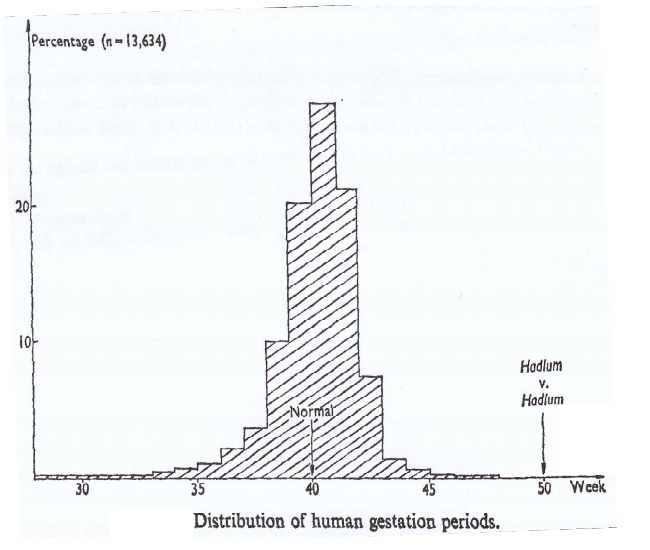
\includegraphics[scale=0.3]{Haldum}
\end{center}
\end{frame}


%------------------------------------------------------------
\begin{frame}\frametitle{Области применения}
\begin{itemize}
\item Поиск мошенничества на основе необычной активности
\item В медицине необычные результаты обследований могут свидетельствовать о потенциальных проблемах со здоровьем
\item Аномальные значения могут быть результатом ошибок в измерении
\item Раннее обнаружение аномальной работы двигателя может предотвратить неожиданную поломку
\end{itemize}
\end{frame}



%--------------------------------------------------------------
\subsection{Попытка формализации}
\begin{frame}\frametitle{Определение аномалии [Howkins, 1980]}
\begin{itemize}
\item Пусть $Q$ некоторый механизм порождения данных
\item $X_1\ldots X_n$ порождены механизмом $Q$
\item $\tilde{X}_1 \ldots \tilde{X}_m$ отличаются от измерений $X_1, \ldots, X_n$, настолько, что можно предположить, что они порождены другим механизмом.
\end{itemize}
\end{frame}

%------------------------------------------------------
\begin{frame}\frametitle{Постановка задачи}

\begin{itemize}
\item $X_1, \ldots, X_N \quad X_i \in S$ -- не размеченная выборка
\item Хотим построить $f \colon S \to \{-1, 1\}$ 
\item $f(X_i) = -1$, если $X_i$ -- аномалия
\item $f(X_i) = 1$, если $X_i$ -- нормальное измерение
\end{itemize}

\end{frame}




%-------------------------------------------------------------
\section{Support Vector Data Description}

\subsection{Оптимизационная задача}
\begin{frame}\frametitle{Support Vector Data Description}
\begin{columns}[T]
\begin{column}{6cm}
\[
\begin{cases}
  R + \frac{1}{N\mathcolor{red}{\nu}}\sum\limits_{i=1}^N\xi_i \to \min\limits_{R, x, \xi}\\
  \| \mathcolor{blue}{\phi}(x_i) - x\|^2 \leqslant R + \xi_i & i = 1,\ldots,N\\
  \xi_i \geqslant 0 & i = 1, \ldots, N\\
  R \geqslant 0
  \end{cases}
 \]
 \begin{itemize}
 \item $\mathcolor{red}{\nu}$ -- верхняя граница количества аномалий и нижняя граница количества опорных векторов
 \item $\mathcolor{blue}{\phi}(x_i)$ -- отображение в пространство более высокой размерности
 \end{itemize}
 \end{column}
\begin{column}{6cm}
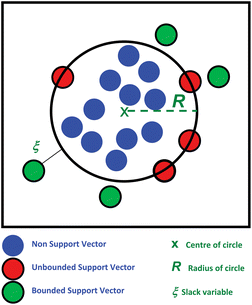
\includegraphics[scale=0.5]{SVDD_explanation.png}
\end{column}
\end{columns}
\end{frame}


\begin{frame}\frametitle{Двойственная задача}
Обычно решают двойственную задачу:
\[
\begin{cases}
\sum\limits_{i=1}^N \alpha_i \phi(x_i)\cdot \phi(x_i) - \sum\limits_{i,j=1}^N\alpha_i \alpha_j \phi(x_i)\cdot \phi(x_j) \to \max\limits_{\alpha} \\
\sum\limits_{i=1}^N \alpha_i = 1\\
0 \leqslant \alpha_i \leqslant \frac{1}{N\nu} \quad i=1,\ldots,N
\end{cases}
\]
Достаточно знать скалярное произведение.
\[
K(x_i, x_j) = \phi(x_i) \cdot \phi(x_j)
\]
\end{frame}

%----------------------------------------------------------
\subsection{Kernel Trick}
\begin{frame}\frametitle{Kernel Trick}
Необязательно знать явный вид спрямляющего пространства, чтобы использовать $K(x, y)$. Достаточно потребовать:
\begin{itemize}
  \item $K(x, y) = K(y, x)$ -- симметричность
  \item $\int_X\int_X K(x, x')g(x)g(x')\text{d}x\text{d}x'$ $\forall g(x)\colon X \to \mathbb{R}$ -- положительная определённость
\end{itemize}
Тогда $K(x,y)$ --  скалярное произведение в некотором пространстве.
\end{frame}


%-----------------------------------------------------------
\begin{frame}\frametitle{Примеры ядер}
\begin{figure}[center]
\begin{tabular}{|c|c|c|}
\hline
Название & Формула & Параметры\\
\hline
Линейное & $x \cdot y$ & ---\\
Полиномиальное & $(\gamma x\cdot y + d)^k$ & $\gamma$, $d$, $k$\\
Гауссово & $\exp(-\gamma\|x - y\|^2)$ & $\gamma$\\
Сигмоидное & $\th(\gamma x\cdot y + d)$ & $\gamma$, $d$\\
\hline
\end{tabular}
\end{figure}
\end{frame}
%------------------------------------------------------------



\begin{frame}\frametitle{Выбор ядрерной функции}
Параметры ядра могут существенно влиять на результат	
\begin{columns}[T]
\begin{column}{6cm}
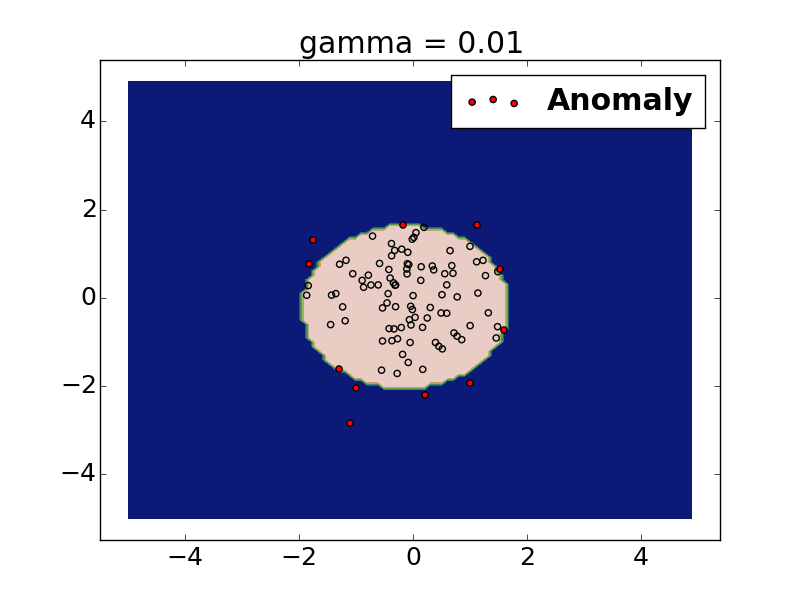
\includegraphics[scale=0.33]{small_gamma.png}
\end{column}
\begin{column}{6cm}
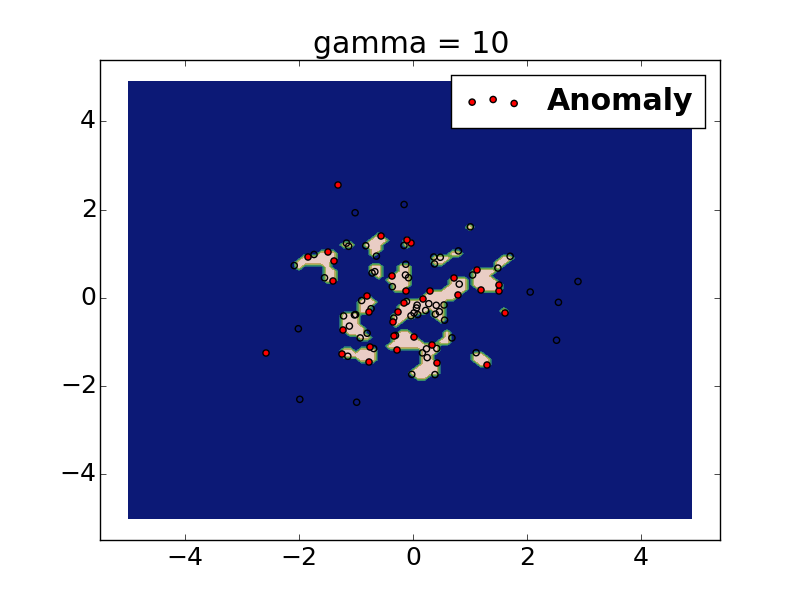
\includegraphics[scale=0.33]{big_gamma.png}
\end{column}
\end{columns}
Хочется получить функцию риска для эффективного подбора параметров ядра.
\end{frame}



%------------------------------------------------------------

\section{Подбор параметров}

\begin{frame}\frametitle{Задача подбора параметров ядра}
\begin{itemize}
\item $X_1, \ldots, X_n$ - обучающая выборка
\item $\gamma$ - параметризация ядра
\item $F(X_1, \ldots, X_n, \gamma)$ -- алгоритм, который по заданной выборке строит классификатор $f(\cdot)$
\item $\tilde{X}_1, \ldots, \tilde{X}_m$ - произвольная тестовая выборка
\item $\tilde{y}_1, \ldots, \tilde{y}_m$ - метки тестовой выборки
\item $\mathcal{R}(f(\cdot), \tilde{X}_1, \ldots, \tilde{X}_m, \tilde{y}_1, \ldots, \tilde{y}_m)$ -- риск ошибки на тестовой выборке
\item Хотим научиться подбирать $\gamma$, не зная тестовую выборку
\end{itemize}
\end{frame}


\subsection{Оптимизация доли опорных векторов и аномалий}
\begin{frame}\frametitle{Оптимизация доли опорных векторов и аномалий}
В приложениях часто пытаются достигнуть границы значений количества аномалий и опорных векторов [Lukashevich et al 2009]
\begin{itemize}
\item $f_{anomaly}$ -- доля объектов отмеченных, как аномалии
\item $f_{support}$ -- доля объектов используемых, как опорные векторы
\end{itemize}
\[
r = (\nu - f_{anomaly})^2 + (\nu - f_{support})^2
\]

\end{frame}	

%---------------------------------------------------------
\subsection{Оптимизация ядерной матрицы}
\begin{frame}\frametitle{Оптимизация функции от ядерной матрицы}
Мерой риска может послужить отношение квадрата стандартного отклонения к среднему значению [Evangelista et al 2007]
\[
r = \frac{s^2}{\bar{k} + \varepsilon}
\]
\[
\bar{k} = \frac{\sum\limits_{i=1}^N\sum\limits_{j=i}^N K(x_i,x_j)}{N(N-1)}; \quad 
s^2 = \frac{\sum\limits_{i=1}^N\sum\limits_{j=i}^N (K(x_i,x_j) - \bar{k})^2}{N(N-1) - 1}
\]
\end{frame}



%--------------------------------------------------
\subsection{Учет распределения аномалий}
\begin{frame}\frametitle{Учет распределения аномалий}
Функция риска может в явном виде учитывать распределения аномальных точек [Steinwart et al 2005]:
\[
r = \frac{1}{(1 + \rho)|S|}\sum\limits_{i\in S}l(1, sign(f(x_i))) + \frac{\rho}{1 + \rho} \mathbb{E}_{\mu}l(-1, sign(f(x_i)))
\]
\[
l(y, t) = \max\{0, 1 - yt\};  \quad \mu \text{ -- распределение аномалий}
\]
Здесь $\rho$ подбирается из априорных соображений.
\end{frame}
%-------------------------------------------------------------
\subsection{Генерация тестовой выборки}
\begin{frame}\frametitle{Генерация тестовой выборки}
Искусственно сгенерируем примеры аномальных и нормальных точек.
\begin{itemize}
\item Аномалии генерируются из равномерного распределения
\item Нормальные данные генерируются на основе тестовой выборки, например при помощи SMOTE (Synthetic Minority Over-sampling Technique)
\end{itemize}
\[
r = \dfrac{1}{|X_{Normal}|}\sum_{x_i\in X_{Normal}} [f(x_i) = -1] + \dfrac{1}{|X_{Anomaly}|}\sum_{x_i \in X_{Anomaly}} [f(x_i) == 1]
\]
\end{frame}


%----------------------------------------------------------



\begin{frame}\frametitle{Synthetic Minority Over-sampling Technique}
\includegraphics{smote}
\end{frame}
%---------------------------------------------------------
\section{Результаты экспериментов}
\subsection{ановка эксперимента}
\begin{frame}\frametitle{Постановка эксперимента}
\begin{itemize}
\item Нормальные данные генерируются из стандартного многомерного нормального распределения

\item Аномалии генерируются из равномерного распределения, причем границы подбираются так, чтобы все нормальные данные попали в заданные границы.

\item Получившиеся данные делятся на обучающую и тестовую выборку. На первой происходит подбор параметров и обучение модели, на второй проверка результата.
\end{itemize}
\end{frame}


%--------------------------------------------------------------
\subsection{Результаты}
\begin{frame}\frametitle{Результаты}
\centering
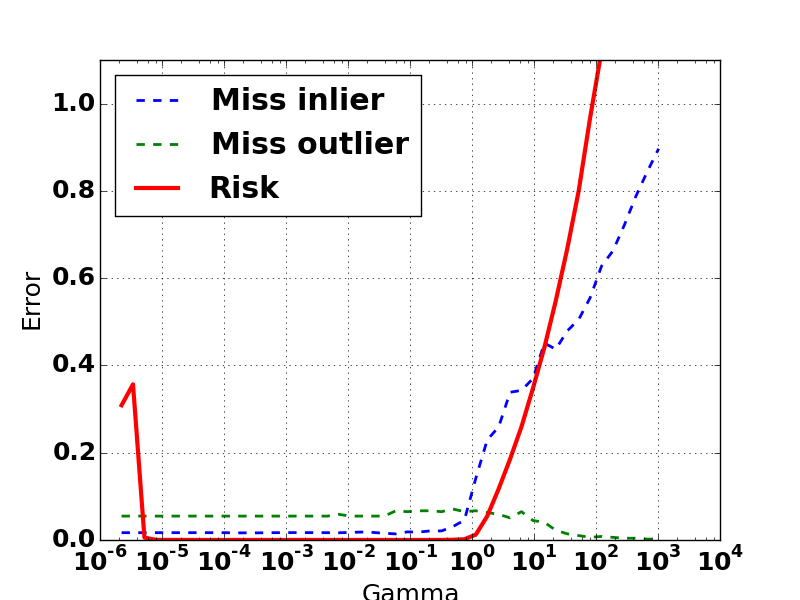
\includegraphics[scale=0.35]{outlier_fraction}\\
Оптимизация количества аномалий и опорных векторов
\end{frame}




\begin{frame}\frametitle{Результаты}
\centering
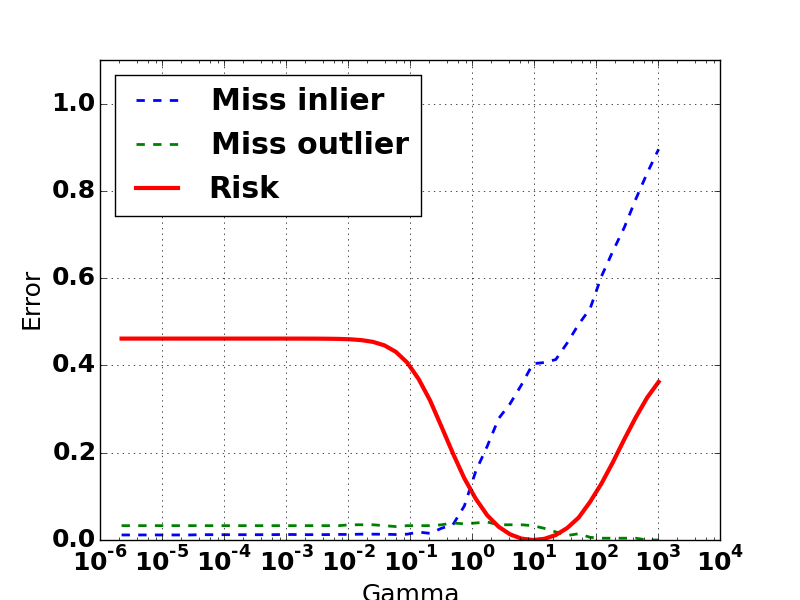
\includegraphics[scale=0.35]{kernel_metric}\\
Оптимизация ядерной матрицы
\end{frame}


\begin{frame}\frametitle{Результаты}
\centering
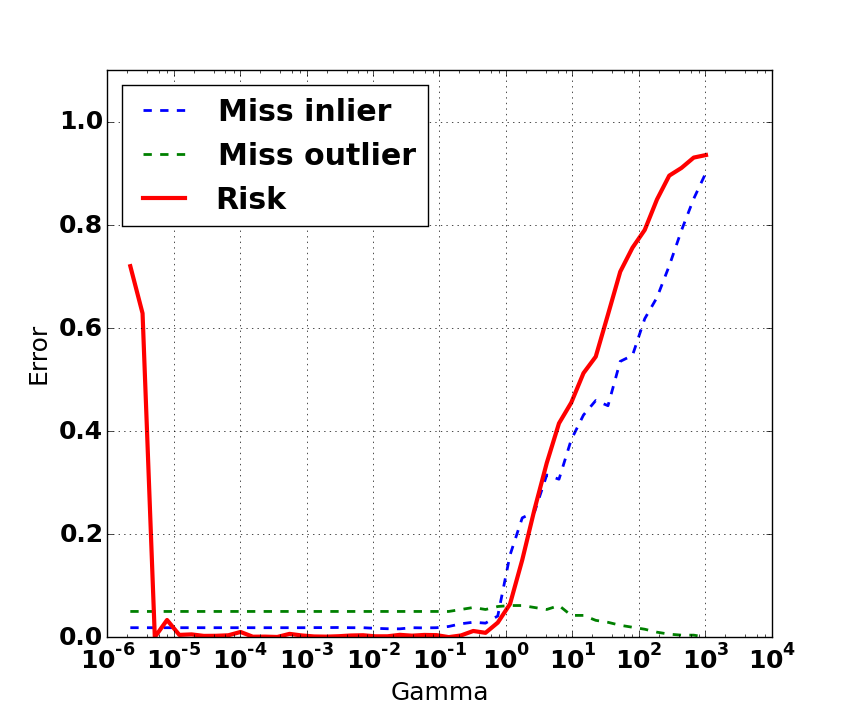
\includegraphics[scale=0.35]{slice_error}\\
Учет распределения аномалий
\end{frame}


\begin{frame}\frametitle{Результаты}
\centering
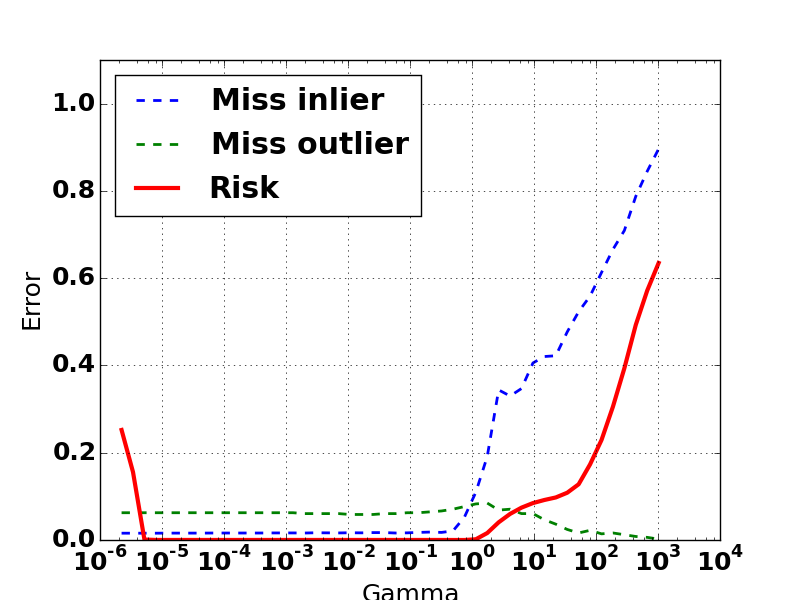
\includegraphics[scale=0.35]{random_generation_metric}\\
Случайная генерация тестовой выборки


\end{frame}

%-------------------------------------------------------------
\begin{frame}\frametitle{Выводы}
\begin{itemize}

\item Только в методе оптимизации ядерной матрицы существует единственный минимум
\item Критерий оптимальности может быть различным в зависимости от важности ошибки на нормальных и аномальных данных
\item Только критерий на основе случайной генерации тестовой выборки способен учитывать различиях ошибок
\end{itemize}
\end{frame}

%------------------------------------------------------------
\begin{frame}
\begin{center}
\Huge{Спасибо за внимание}
\end{center}
\end{frame}
\end{document}